\documentclass[oneside,a4paper,12pt]{article}
% ---------------- Para Modificar ---------------- 
\newcommand{\principal}{Volumes}
\newcommand{\conteudo}{}
\newcommand{\turmas}{3~EMSI~A e do 3~EMSI~B}

\date{abril de 2021}

\newcommand{\citacao}{Que nada nos defina. Que nada nos sujeite. Que a liberdade seja a nossa própria substância.}
\newcommand{\autorcitacao}{Simone de Beauvoir}
% ------------------------------------------------

%-------------------------------------------------
\usepackage[english,brazilian]{babel}
\usepackage[alf]{abntex2cite}
\usepackage[utf8]{inputenc}
\usepackage[T1]{fontenc}
\usepackage[top=15mm, bottom=15mm, left=10mm, right=10mm]{geometry}
\usepackage{framed,booktabs,color,hyperref,graphicx}
\usepackage{amsfonts,amsthm,cancel}
\usepackage{subfigure,enumerate,float}
  
\definecolor{shadecolor}{rgb}{0.8,0.8,0.8}
\pagenumbering{arabic}

% Colunas
\usepackage{multicol}
\columnsep=10mm %Espaçamento entre colunas.
\setlength{\columnseprule}{1pt}

% Cabeçalho
\usepackage{fancyhdr}
\pagestyle{fancy}
\lhead{\textbf{\principal}}
\rhead{}
\renewcommand{\headrulewidth}{1pt} % espessura da linha do cabeçalho
\renewcommand{\footrulewidth}{1pt} % espessura da linha do rodapé

% Parágrafo
\setlength{\parindent}{1.25cm}

\newtheorem{problema}{Problema}
\newtheorem{exercicio}{exercicio}
\newtheorem{exemplo}{Exemplo}
\newtheorem{questao}{Questão}

\usepackage[skip=10pt]{caption}
\captionsetup{font={stretch=0.4,small}}

\newcommand{\FRASE}{\textit{``\citacao ''}\\(\textbf{\autorcitacao})}

\title{\LINHAHORIZONTAL \\\textbf{\\ \principal}\footnote{Resumo para os estudos das aulas não presenciais no período de quarentena para as turmas do \turmas .}\\\LINHAHORIZONTAL}

\newcommand{\LINHAHORIZONTAL}{\center \rule{16cm}{1.25pt}}
\newcommand{\sol}{\textbf{Solução}}

\newcommand{\m}[1]{\(\displaystyle {#1}\)}
\newcommand{\M}[1]{\[{#1}\]}

\author{\textbf{Professor Leandro Vieira}\\EREM Regina Pacis\\Palmeirina-PE}
\newcommand{\frase}{\begin{verse} \flushright{\FRASE} \end{verse}}


\begin{document}
\begin{enumerate}

\item O Butão é um país localizado no sul da Ásia, no extremo leste dos Himalaias. Faz fronteira ao norte com a China e ao sul, leste e oeste com a índia. A seguir é apresentada uma tabela com informações sobre as cidades mais populosas do Butão:

\begin{figure}[!hbt]
\begin{multicols}{2}
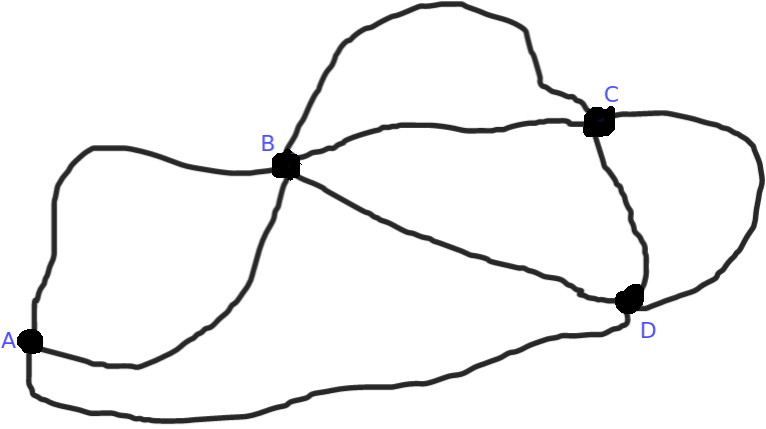
\includegraphics[width=8cm]{03}

\columnbreak
Com base nas informações apresentadas na tabela, sabendo que a população do Butão é de 831 557 , resolva os itens a seguir:
\begin{enumerate}
\item 

\item 
\end{enumerate}

\end{multicols}
\end{figure}

\item A Tabela~\ref{tabela1} a seguir traz dados sobre a taxa de homicídios a cada 100 mil pessoas por ano em algumas unidades federativas dos Estados Unidos.

\begin{table}[htb]
\center
\begin{tabular}{p{1cm}lrc}
\hline 
 & \textbf{Estado} & \textbf{População} & \textbf{Taxa de Homicídio} \\ 
\hline 
1 & Alabama & 4.779.736 & 5,7 \\ 

2 & Alasca & 710.231 & 5,6 \\ 
 
3 & Arizona & 6.392.017 & 4,7 \\ 
 
4 & Arkansas & 2.915.918 & 5,6 \\ 

5 & Califórnia & 37.253.956 & 4,4 \\ 

6 & Colorado & 5.029.196 & 2,8 \\ 

7 & Connecticut & 3.574.097 & 2,4 \\ 

8 & Delaware & 897.934 & 5,8 \\ 
\hline
\end{tabular} 
\caption{} 
\label{tabela1}
\end{table}
Com base nas informações apresentadas na questão e na tabela anterior responda aos seguintes itens:
\begin{enumerate}
\item Qual dos estados apresentados tem a maior população?
\item Qual dos estados tem a menor taxa de homicídios?
\item Qual o número de homicídios no estado do Colorado?
\item Qual o número de homicídios no estado que tem a menor população?
\item Qual a taxa de homicídios e a taxa de homicídios no estado do Arkansas?
\item Com base nas informações apresentadas na tabela crie uma gráfico para a taxa de homicídios por estado, e outro para o número para a população por estado:

\end{enumerate}

\end{enumerate}
\end{document}